\documentclass[a4paper, 12pt]{article}
\usepackage[margin=1in]{geometry}
\usepackage{socstyle}
\def\asydir{../../asy}
\usepackage[]{pdfpages}

\usepackage[backend=biber, url=true, sorting=none]{biblatex}
\usepackage{url}
\addbibresource{/home/adam/tex/soc.bib}

\begin{document}
\pagestyle{empty}
{\centering \section*{\Huge Mechanika rodin planetek\\s aplikací na rodinu Eunomia}
\textbf{Adam Křivka}
\subsection*{\LARGE Synopse}}

\vfill

\renewcommand{\baselinestretch}{0.75}\normalsize
\tableofcontents
\renewcommand{\baselinestretch}{1.3}\normalsize

\vfill
\textbf{Adam Křivka\\
Cyrilometodějské gymnázium\\ a střední odborná škola pedagogická Brno \hfill Brno, 2019}
\newpage

\section{Planetky ve sluneční soustavě}
Planetky jsou nejpočetnější a svým způsobem nejzajímavější skupinou těles ve~sluneční soustavě. První planetka byla objevena v roce 1801, v dnešní době je již známo přes půl milionu planetek.

V~hlavním pásu planetek mezi \textit{Marsem} a~\textit{Jupiterem} tvoří planetky rodiny --- skupiny vzniklé rozpadem stejného mateřského tělesa, způsobeným srážkou s~jiným tělesem. V~naší práci se soustředíme na početnou rodinu \textit{Eunomia}, nacházející se ve středním hlavním pásu.

Studiem kolizních rodin můžeme zjistit mnoho informací o~vzniku sluneční soustavy a~její dynamické struktuře, např. můžeme podpořit teorii o~Velkém pozdním bombardování (angl. \textit{Late Heavy Bombardment}).
\newpage

\begin{figure}[!ht]
	\centering
	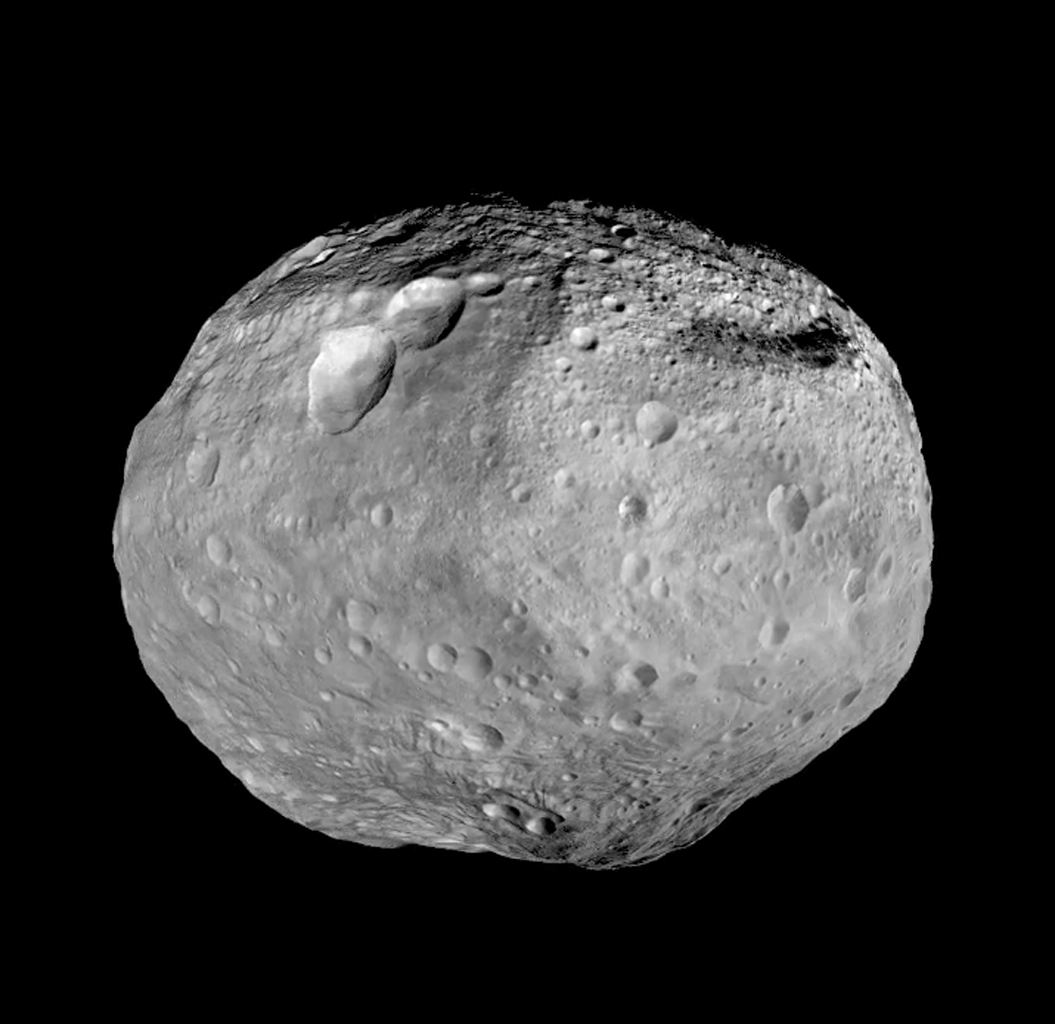
\includegraphics[width=0.6\textwidth]{../../obr/vesta.jpg}
	\caption{Planetka \textit{(4) Vesta} --- druhé největší a~nejhmotnější těleso hlavního pásu planetek.} 
	\label{fig:vesta}
\end{figure}
\begin{figure}[!hb]
	\centering
	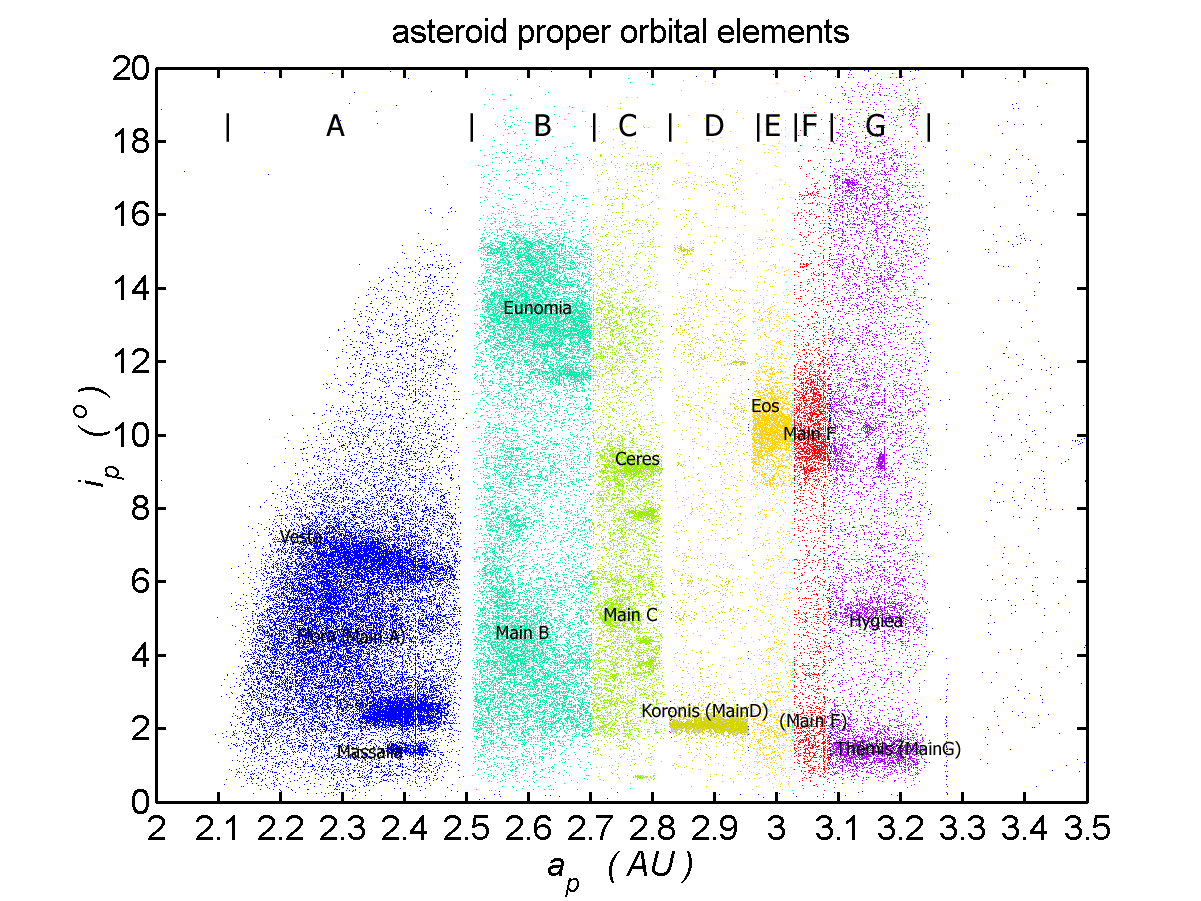
\includegraphics[width=0.8\textwidth]{../../obr/mainbelt.png}
	\caption{Hlavní pás planetek v prostoru vlastních elementů dráhy --- vlastní hlavní poloosy $a_{\rm p}$ vlastní sklon $\sin I_{\rm p}$.} \label{fig:belt}
\end{figure}

\section{Nebeská mechanika}

\subsection{Problém $N$ těles}
Základním problémem nebeské mechaniky je problém $N$ těles --- pomocí pohybových rovnic dle Newtonova gravitačního zákona určit polohy $N$ těles v čase, podle vztahu

\begin{align*} 
	\vec{F}_i = m_i\vec{a}_i &= -\sum_{\substack{j=1 \\ j\neq i}}^N G\frac{m_im_j}{\abs{\vec{r}_i-\vec{r}_j}^3}(\vec{r_i}-\vec{r_j})\,, \qquad{\rm pro}\ i\in\{1,\,2,\,\dots,\,N\}\,.
\end{align*}}

\begin{figure}
	\centering 
	\begin{subfigure}[b]{0.45\textwidth}
	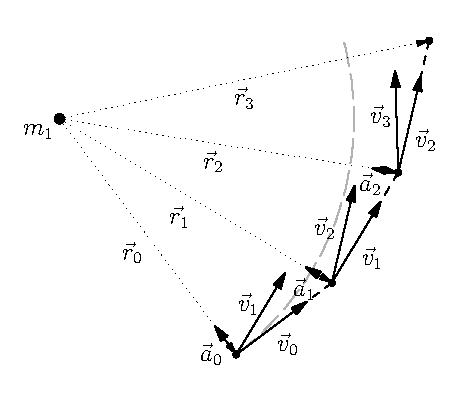
\includegraphics[width=1.0\textwidth]{../../asy/asteroidy-3.pdf}
	\end{subfigure}
	\begin{subfigure}[b]{0.45\textwidth}
	\centering 
	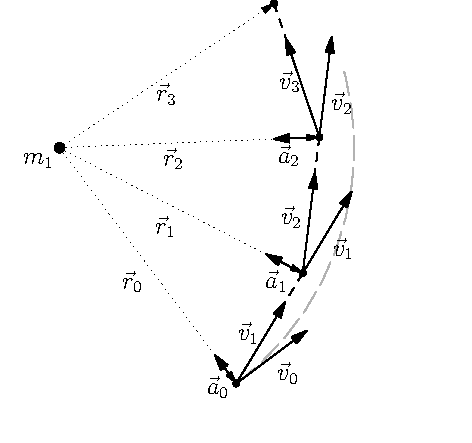
\includegraphics[width=1.0\textwidth]{../../asy/asteroidy-4.pdf}
	\end{subfigure}
	\caption{Ilustrace jednodušší integrační metody --- Eulerovy metody --- která je pricipielně té naší podobná.}
	% \caption{Ilustrace dopředné Eulerovy integrační metody pro dvě tělesa. Jsou ukázány první tři iterace. Šedá křivka znázorňuje analytické řešení problému dvou těles.} \label{fig:euler}
\end{figure}
\vspace{-1cm}
\subsection{Numerický integrátor}

K řešení problému $N$ těles a k simulaci orbitálního vývoje využíváme symplektického numerického integrátoru SWIFT, který počítá i s 

\begin{itemize}
\itemsep0em
\item \textbf{Jarkovského jevem} (nerovnoměrné vyzařování tepla zrychlující/zpomalující planetku --- změna hlavní poloosy),
\item \textbf{YORP efektem} (nerovnoměrné vyzařování tepla ovlivňující rotační osu planetky),
\item \textbf{náhodnými srážkami},
\item \textbf{chaotickou difuzí}.  
\end{itemize}

\subsection{Elementy dráhy}
Oběžnou dráhu planetky kolem Slunce popisujeme především těmito elementy dráhy (dohromady jich je ale šest):
\begin{itemize}
	\itemsep0em
	\item \textbf{hlavní poloosa} $a$
	\item \textbf{excentricita} $e$
	\item \textbf{sklon} $I$ (nebo také $\sin I$) 
\end{itemize}

Elementy dráhy se v průběhu času mění působením perturbací (např. gravitačním působením ostatních planet), můžeme je tedy přes dlouhé úseky zjedondušeně řečeno \uv{průměrovat} na střední a na vlastní elementy dráhy. Pro popis rodin planetek se nejčastěji používají vlastní elementy dráhy, protože nepodléhají téměř žádným periodickým perturbacím.

\begin{figure}
	\centering
	\includegraphics[width=0.7\textwidth]{../../obr/atOF}
	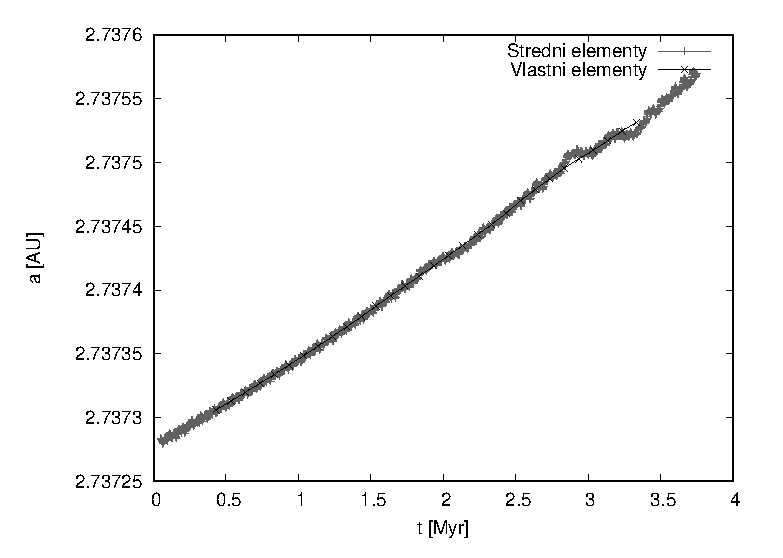
\includegraphics[width=0.7\textwidth]{../../obr/atFP}
	\caption{Porovnání oskulační (aktuální) a střední hlavní poloosy (vlevo) a střední a~vlastní hlavní poloosy (vpravo) pro simulaci jedné planetky po dobu $3,76$ miliónů let.}
\end{figure}


\subsection{Určení rodiny}
K určení členů rodiny používáme hierarchickou shlukovací metodu (HCM) --- v prostoru $(a_{\rm p},\,e_{\rm p},\sin I_{\rm p})$ si zvolíme hraniční vzájemnou \uv{vzdálenost} těles $v_{\rm cutoff}$ (s jednotkami rychlosti)
\begin{align*}
	v_{\rm cutoff}=na_{\rm p}\sqrt{C_a\left(\frac{\Delta a_{\rm p}}{a_{\rm p}}\right)^2+C_e(\Delta e_{\rm p})^2+C_i(\Delta \sin i_{\rm p})^2}\,,
\end{align*}
podle které pak určíme členy (začneme u mateřského tělesa \textit{(15) Eunomia}) --- pokud je vzdálenost dalšího tělesa menší, než $v_{\rm cutoff}$, přidáme jej do rodiny.

\begin{figure}
	\centering
	\includegraphics[width=0.7\textwidth]{../../obr/Nv_edit.png}
	\caption{Závislost počtu členů rodiny \textit{Eunomia} na zvolené hraniční rychlosti $v_{\rm cutoff}$ při použití metody HCM. Počet členů prudce vzroste při přechodu z~$43$ na $44\,{\rm m/s}$, což je způsobené velkou vzdáleností prvního nejbližšího tělesa od mateřského \textit{(15) Eunomia}. Dále vzroste prudce při přechodu z~$46$ na $47\,{\rm m/s}$, což je způsobené splynutím s~rodinou Adeona.}
\end{figure}
\clearpage

\newpage
\section{Vlastnosti rodiny Eunomia}

\subsection{Určení rodiny}
K určení rodiny \textit{Eunomia} jsme použili metodu HCM. Dále jsme odstranili přimísená tělesa pomocí závislosti unášení ve vlastní hlavní poloose $\Delta a_{\rm p}$ na absolutní hvězdné velikosti $H$ a pomocí dvou spektroskopických metod --- závislosti albed $p_{\rm V}$ a $p_{\rm IR}$ a závislosti barevných indexů $a^*$ a $i-z$. Před odstraněním činil počet planetek 6503, po použití všech metod~6184.

\begin{figure}
	\centering
	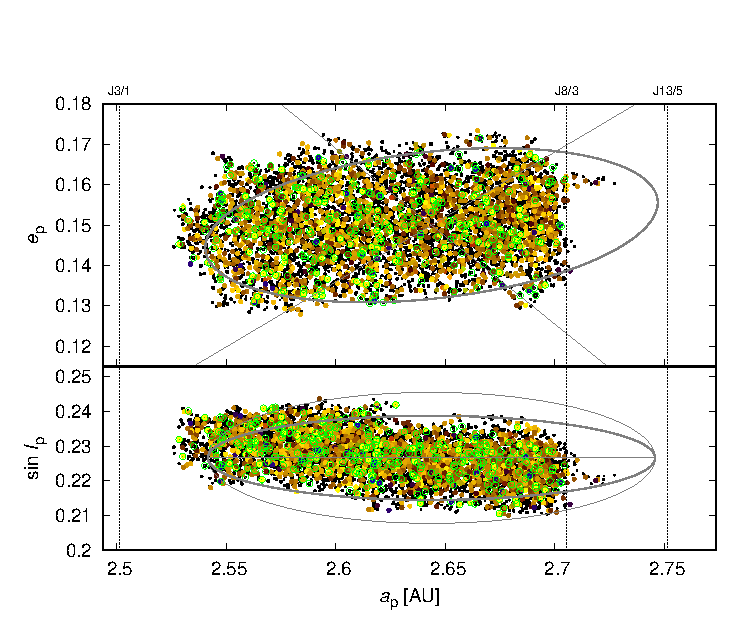
\includegraphics[width=0.9\textwidth]{../../obr/ae_ai_wise}
	\caption{Pozorovaná rodina \textit{Eunomia} určená HCM s hodnotou $v_{\rm cutoff} = 44\,{\rm m/s}$ v~rovině vlastní hlavní poloosy $a_{\rm p}$ a~vlastní excentricity $e_{\rm p}$ (nahoře) a~v~rovině vlastní hlavní poloosy $a_{\rm p}$ a~vlastního sklonu $\sin I_{\rm p}$ (dole). Barevná škála odpovídá albedu $p_{\rm V}$ a~$p_{\rm IR}$ z~katalogu WISE.}
% Nápisy J3/1, J8/3 a~J13/5 označují polohu rezonancí středního pohybu s~\textit{Jupiterem}. Šedé elipsy a~úsečky (degenerované elipsy) naznačují předpokládaný tvar rodiny, při rozpadu v bodě oběžné dráhy s hodnotami pravé anomálie $f=0^\circ,\,90^\circ,\,180^\circ$ (nahoře) a~jejího součtu s argumentem pericentra $\omega+f=0^\circ,\, 50^\circ,\, 90^\circ$ (dole), kde elipsou zvolenou pro další výpočety je elipsa pro hodnoty $f=90^\circ$ a~$\omega+f=50^\circ$.
	\label{fig:ae_ai_wise}
\end{figure}
\begin{figure}
	\centering
	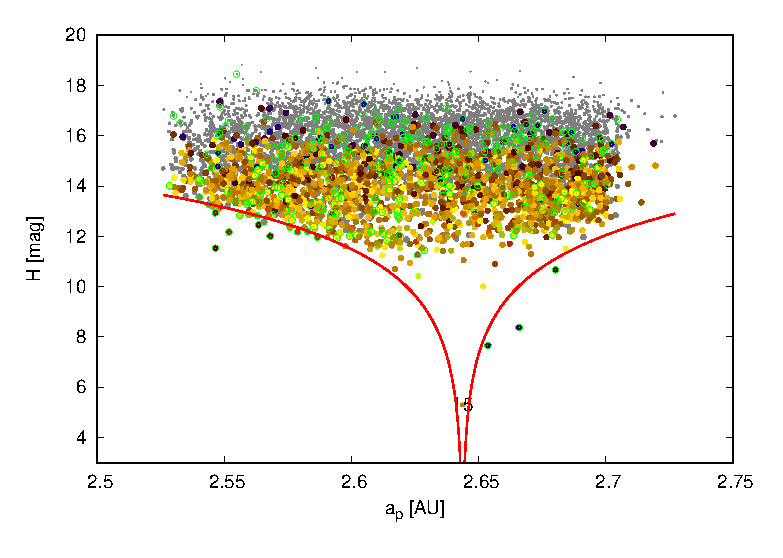
\includegraphics[width=0.9\textwidth]{../../obr/aH_wise}
	\caption{Závislost unášení ve vlastní hlavní poloose $a_{\rm p}$ na~absolutní hvězdné velikosti $H$. Lze pozorovat typický tvar \uv{V}, který je způsoben počátečním rychlostním polem a~Jarkovského jevem, jenž je ještě zesílen vlivem YORPu, což způsobuje zvýšenou koncentraci malých planetek při okrajích rodiny.\newline\newline}
\end{figure}
\begin{figure}
	\centering
	\includegraphics[width=0.65\textwidth]{../../obr/pV_pIR-crop}
	\caption{Albeda $p_{\rm V}$ (ve viditelném spektru) a~$p_{\rm IR}$ (v~infračerveném) z~katalogu WISE. Barvy neodpovídají reálnému zbarvení. Pro vyřazení přimísených těles touto metodou byly zvoleny hraniční hodnoty $0,05 \leq p_{\rm V} \leq 0,4$.\newline}
	\centering
	\includegraphics[width=0.65\textwidth]{../../obr/astar_iz-crop}
	\caption{Barevné indexy $a^*$ a~$i-z$ z~katalogu Sloan. Barvy neodpovídají reálnému zbarvení. Pro vyřazení přimísených těles byly zvoleny hraniční hodnoty $0\leq a^* \leq 0,3$ a~$-0,3\leq i-z \leq 0,3$.\newline\newline}
\end{figure}
\clearpage

\subsection{Simulace orbitálního vývoje}

Při vytváření syntetické populace planetek jsme částicím přiřadili 
\begin{itemize}
\itemsep0em
\item \textbf{průměry} (dle pozorovaných dat --- zohlednili jsme rozdělení velikostí), 
\item \textbf{albeda} (dle pozorovaných dat),
\item \textbf{orientace rotačních os} (náhodně; vliv na Jarkovského jev),
\item \textbf{úvodní rychlosti} (jako při izotropním rozpadu v bodě oběžné dráhy s hodnotami $f=90^\circ$ a $\omega+f=50^\circ$).
\end{itemize}
% . U průměrů jsme zohlednili rozdělení velikostí a při zpracovávání simulace jsme rozdělení korigovali tak, aby odpovídalo pozorovanému.


Po dobu $1,3$ miliardy let jsme simulovali populaci 6210 částic. Simulace byla spuštěna na výpočetním clusteru Astronomického ústavu Univerzity Karlovy a celkově se spotřebovalo přibližně 50000 CPU hodin a celkový objem binárních dat je roven $164\,{\rm GB}$.

\begin{figure}
	\centering
	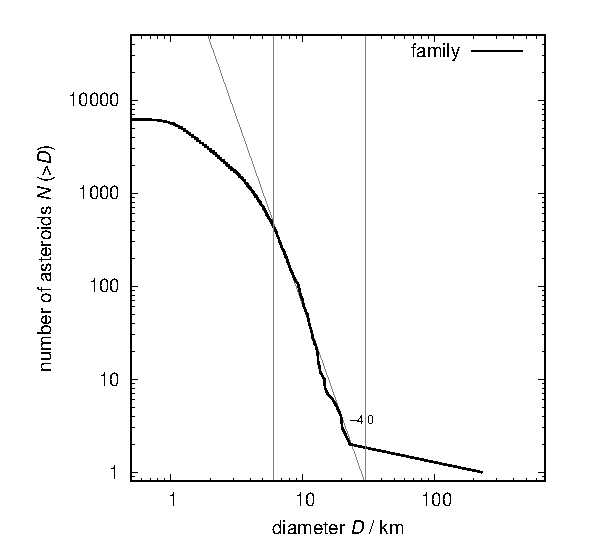
\includegraphics[width=0.6\textwidth]{../../obr/size_distribution}
	\caption{Histogram četnosti velikostí planetek rodiny \textit{Eunomia}.} 
% kde veličina $N({>}D)$ označuje počet planetek s~průměrem větším než $D$.
%Jedná se o~logaritmický graf $(\log D,\,\log N({>}D))$, na kterém lze vztah mezi danými veličinami aproximovat přímkou, což znamená, že vztah mezi veličinami $D$ a~$N({>}D)$ je mocninný.}

% Vodorovná část zcela vlevo je způsobena observační nedostatečností. Změna sklonu přímky prvního intervalu $D$ (vlevo, $q=-4$) na druhý interval $D$ (vpravo, $q=-1,2$) je důsledkem jednak prvotního rozpadu a~jednak druhotného vývoje --- tělesa se nadále srážejí, vytvářejí menší tělesa, která snáze opouštějí rodinu.
	\label{fig:sfd}
\end{figure}

\subsection{Výsledky simulace}

Následující závěry se pojí k obrázkům \ref{fig:vysledky1}, \ref{fig:vysledky2}, \ref{fig:vysledky3}.

\begin{figure} 
	\centering
	\includegraphics[width=0.49\textwidth]{../../obr/ae_5.png}
	\includegraphics[width=0.49\textwidth]{../../obr/ae_205.png}\\
	\includegraphics[width=0.49\textwidth]{../../obr/ae_605.png}
	\includegraphics[width=0.49\textwidth]{../../obr/ae_1105.png}
		\caption{Výsledky simulace v~prostoru $(a_{\rm p},\,e_{\rm p})$ v~časech postupně $t=5,\,205,\,605,\,1105$ miliónů let. Nápisy J3/1, J8/3, J13/5 a~J5/2 označují nejvýznamnější rezonance s~\textit{Jupiterem}. Černá křivka nahoře označuje hranici oblasti, kde je hlavní poloosa a~excentricita tělesa taková, že dráha kříží dráhu \textit{Marsu}. Podobná hranice existuje i~pro Jupiter, ale ta se nachází mimo tyto grafy (přibližně kolem $e=0,65$).} \label{fig:vysledky1}
\end{figure}
\begin{figure} 
	\includegraphics[width=0.49\textwidth]{../../obr/ai_5.png}
	\includegraphics[width=0.49\textwidth]{../../obr/ai_205.png}\\
	\includegraphics[width=0.49\textwidth]{../../obr/ai_605.png}
	\includegraphics[width=0.49\textwidth]{../../obr/ai_1105.png}
		\caption{Výsledky simulace v~prostoru $(a_{\rm p},\,\sin I_{\rm p})$ v~časech postupně $t=5,\,205,\,605,\,1105$ miliónů let. Nápisy J3/1, J8/3, J13/5 a~J5/2 označují nejvýznamnější rezonance s~\textit{Jupiterem}.} \label{fig:vysledky2}
\end{figure}
\begin{figure}
	\includegraphics[width=0.49\textwidth]{../../obr/ei_5.png}
	\includegraphics[width=0.49\textwidth]{../../obr/ei_205.png}\\
	\includegraphics[width=0.49\textwidth]{../../obr/ei_605.png}
	\includegraphics[width=0.49\textwidth]{../../obr/ei_1105.png}
		\caption{Výsledky simulace v~prostoru $(e_{\rm p},\,\sin I_{\rm p})$ v~časech postupně $t=5,\,205,\,605,\,1105$ miliónů let. Fialový obdélník označuje oblast vybranou pro vzorek populace pozadí.} \label{fig:vysledky3}
\end{figure}

\begin{itemize}
\item 
Kvůli specifickému výpočtu vlastních elementů dráhy z~počátečních rychlostí můžeme v~čase 5 miliónů let pozorovat mírně nesymetrický tvar simulované~rodiny. 

\item Mechanismus, kterým planetky opouštějí rodinu je následovný: působením Jarkovského jevu se planetka dostane do blízkosti nějaké rezonance, excentricita její oběžné dráhy se zvýší až začne křížit dráhu \textit{Marsu} nebo \textit{Jupiteru}, načež se pak při blízkém přiblížení prudce vychýlí ze své dráhy.

\item 
Tělesa nacházející se na počátku v blízkosti rezonance J5/2 byla velmi rychle rozptýlena, a tak se už na grafu pro $t=5$ miliónů let vůbec nevyskytují.

\item
Rezonance J8/3 a~J13/5 jasně rozdělují rodinu na tři části, které různě široké, a tudíž se v nich planetky rozptylují jinak.

\item 
Potvrzuje se, že rezonance J8/3 je silnější než rezonance J13/5 (planetky v~blízkosti rezonance J8/3 se v~čase 205 miliónů let rozšířily do pásu o~velikosti $0,05<e_{\rm p}<0,5$, zatímco v~blízkosti rezonance J13/5 pouze do pásu o~velikosti $0,1<e_{\rm p}<0,23$)

\item
Na grafu $(a_{\rm p},\,\sin I_{\rm p})$ můžeme pozorovat mírné \uv{naklonění} pozorované rodiny (část pod $a\approx2,62\,{\rm AU}$ má vyšší sklon $I_{\rm p}$), čehož si na rodině simulované bohužel zatím všimnout nemůžeme.

\item Postupem času koncentrace planetek v prostoru klesá, což je způsobeno všemi přítomnými rezonancemi.

% Lze vidět vliv rezonancí středního pohybu J3/1, J5/2, J8/3 a J13/5 --- v jejich blízkosti se excentricity planetek začnou zvyšovat, až se dostanou do oblasti, kde kříží dráhy \textit{Marsu} nebo \textit{Jupitera}, což znamená, že se planetka dříve nebo později některé z~těchto planet přiblíží a~její hlavní poloosa se náhle změní. Na prvním obrázku jsou data již zprůměrována z~prvních $10$ miliónů let, takže můžeme vidět, že se planetky, které se zřejmě na počátku nacházely v~blízkosti rezonancí J3/1, J8/3 a~J13/5, stihly rozptýlit a~narušily tak jinak zatím pravidelný tvar rodiny. 

\end{itemize}

\begin{figure}
	\centering
	\includegraphics[width=0.6\textwidth]{../../obr/ae_obs.png}
	\caption{Graf $(a_{\rm p}, e_{\rm p})$ pro pozorovanou rodinu \textit{Eunomia}. Barevná škála označuje počet těles v~daném boxu.}
% Vpravo v oblasti $a_{\rm p}\in(2,7\,{\rm AU};\,2,75\,{\rm AU}),\ e_{\rm p}\in(0,16;\,0,18)$ lze pozorovat velmi malou rodinu příslušnou planetce $(53546)\ 2000\,BY6$, se kterou jsme v~naší simulaci, stejně jako s~ostatními rodinami, nepočítali.
	\centering
	\includegraphics[width=0.49\textwidth]{../../obr/ae_scl_0006.png}
	\includegraphics[width=0.49\textwidth]{../../obr/ae_scl_0206.png}\\
	\includegraphics[width=0.49\textwidth]{../../obr/ae_scl_0606.png}
	\includegraphics[width=0.49\textwidth]{../../obr/ae_scl_1106.png}
	\caption{Graf $(a_{\rm p},\,e_{\rm p})$ simulované rodiny Eunomia pro $t=5,\ 205,\ 605, 1105$ miliónů let. Pozor na změnu barevné škály.} 

	\label{fig:ae_chi2}
\end{figure}
\clearpage

\section{Diskuze} 
\subsection{Metoda blackbox}

Planetky jak pozorované, tak simulované rodiny rozdělíme do \uv{boxů} v~prostoru $(a_{\rm p},\,e_{\rm p},\,\sin I_{\rm p})$ a~následně porovnáváme počty planetek v~jednotlivých boxech. Simulovanou populaci ještě \uv{smícháváme} se vzorkem pozadí, přičemž dodržujeme rozdělení velikostí. 

Na tento jednoduchý princip pak používáme statistickou metodu rozdělení chí kvadrátu ($\chi^2$) --- pro každý box vypočteme jeho příspěvek k~$\chi^2$ jako
\begin{align*}
	\frac{(N_{\rm sim}-N_{\rm obs})^2}{N_{\rm sim}+N_{\rm obs}}\,.
\end{align*}

% kde $N_{\rm sim}$, resp.\ $N_{\rm obs}$ označuje počet simulovaných, resp. pozorovaných těles v~daném boxu. Výslednou hodnotu $\chi^2$ potom dostaneme prostým sečtením všech příspěvků.\begin{figure}
	\begin{figure}
	\centering
	\includegraphics[width=0.49\textwidth]{../../obr/ae_chi_0006.png}
	\includegraphics[width=0.49\textwidth]{../../obr/ae_chi_0206.png}\\
	\includegraphics[width=0.49\textwidth]{../../obr/ae_chi_0606.png}
	\includegraphics[width=0.49\textwidth]{../../obr/ae_chi_1106.png}
	\caption{Hodnota chí kvadrátu $\chi^2$ pro každý box v~prostoru $(a_{\rm p},\,e_{\rm p})$ pro $t=5,\ 205,\ 605,\ 1105$ miliónů let. Tečky označují syntetickou populaci i~s~přidaným pozadím.} 
	\label{fig:ae_chi2}
	\end{figure}

\subsection{Závěry}

Můžeme vidět, že ze začátku se nejvíce odlišuje jádro rodiny kolem $2,65\,{\rm AU}$ (moc syntetických částic).   

Kvůli silné kontaminaci rodinou \textit{Adeona} v oblasti $0,16<e<0.18$ jsme byli nuceni pozorované členy této rodiny ručně odstranit.

Podařilo se nám pochopit struktur, které lze na našich grafech v prostorech $(a_{\rm p},\,e_{\rm p})$, $(a_{\rm p},\,\sin I_{\rm p})$ a  $(e_{\rm p},\,\sin I_{\rm p})$. Některé jevy (např. přílišná kompaktnost jádra) bohužel musíme připsat nedostatečně dlouhému časovému úseku, po který jsme rodinu \textit{Eunomia} simulovali. S velkou pravděpodobnstí můžeme říct, že rodina \textit{Eunomia} není mladší než $500$ miliónů let, ale zatím nedokážeme odhadnout (z důvodu ploché závislosti chí kvadrátu na čase), jaký je horní limit stáří rodiny Eunomia.


	\begin{figure}
		\centering
		\includegraphics[width=0.6\textwidth]{../../obr/chi2.eps}
		\caption{Závislost redukovaného chí kvadrátu na čase. Skok v čase přibližně 1125~miliónů let je způsoben úbytkem těles v simulaci.}
	\end{figure}


\subsection{Budoucí práce}

V~budoucnu plánujeme simulovat rodinu \textit{Eunomia} po delší dobu (4 miliardy let). Pravděpodobně dostaneme nějakou minimální (statisticky významnou) hodnotu chí kvadrátu, čímž budeme schopni přesně určit horní mez pro stáří rodiny \textit{Eunomia}.   

Další možností vylepšení je analýza okolních rodin, zejména rodiny \textit{Adeona}. %Přesné určení počtu jejích členů a~stáří by nám pomohlo v~analýze rodiny \textit{Eunomia}, mohli bychom např. v~momentu rozpadu rodiny \textit{Adeona} její částice do simulace přidat.
Můžeme se také zaměřit jen na některé taxonomické typy planetek (rodina \textit{Eunomia} je typu S) nebo vyzkoušet anizotropní rychlostní pole --- simulovat různé typy rozpadu (kráterování, reakumulace, katastrofický rozpad). Dále můžeme vyzkoušet různé vzorky pozadí pro různé oblasti (mezi rezonancemi J8/3 a J13/5 je menší koncentrace pozorovaných těles než mezi rezonancemi J3/1 a J8/3).

Po dokončení dlouhodobé simulace plánujeme publikaci výsledků v~odborném časopisu (\textit{Icarus}).


% \includepdf[pages={52,53,54}]{../../asteroidy.pdf}

\end{document}
